\documentclass{article}
%\usepackage{geometry}
% \geometry{top = 1in, bottom = 1in, left = 1in, right = 1in}
\usepackage[top = 0.7in, bottom = 0.7in, left = 0.7in, right = 0.7in]{geometry}
\usepackage{amsmath,amssymb,amsthm,mathrsfs}
\usepackage{graphicx}
\usepackage{bm}
\usepackage{float}
\usepackage[font=footnotesize,labelfont=bf]{caption}

\usepackage{fancyhdr}
\pagestyle{fancy}
\rhead{\footnotesize {07/26/2012 ; MESA version 4161} }
\chead{\footnotesize \parbox{6cm}{Authors: Jared Brooks, Matteo \newline Cantiello, Lars Bildsten, Bill Paxton} }
\lhead{\footnotesize {mesa/star/test\_suite/15M\_dynamo} }

\begin{document}
	
	\begin{center}
		\begin{Large}
		       \textbf{15M DYNAMO}\\
		\end{Large}
	\end{center}

        This test is to show the capability of \texttt{MESA} to deal with rotating stars. It evolves a slowly-rotating (initially 1\% of surface critical rotational rate) 14.4 $M_\odot$ star during core He burning.  During the evolution the transport of angular momentum and chemicals due to the presence of rotational instabilities is accounted for in a diffusion approximation.  Magnetic mixing in radiative regions produced by the Spruit-Tayler dynamo is also considered.  The test should be cut off when the mass fraction of center helium drops below 0.2 (\texttt{xa\_central\_lower\_limit\_species(1) = 'he4' ; xa\_central\_lower\_limit(1) = 0.2}).  To verify that this test ran successfully, \texttt{MESA} checks a set of parameters to see if they fall inside a range of expected values, listed in \texttt{src/run\_star\_extras.f}.  If all the parameter values fall within their respective ranges, the terminal output at the end of the run should read \texttt{``all values are within tolerances''}.\\

        The star is evolved for about 830,000 years. During this period it loses mass and angular momentum through a stellar wind (figure \ref{fig:1}).  Its evolution on the HR-diagram is shown in figure \ref{fig:2}, starting on the top branch and ending at a lower luminosity.

	\begin{figure}[H]
                \begin{minipage}[b]{0.5\linewidth}
		       \centering
		       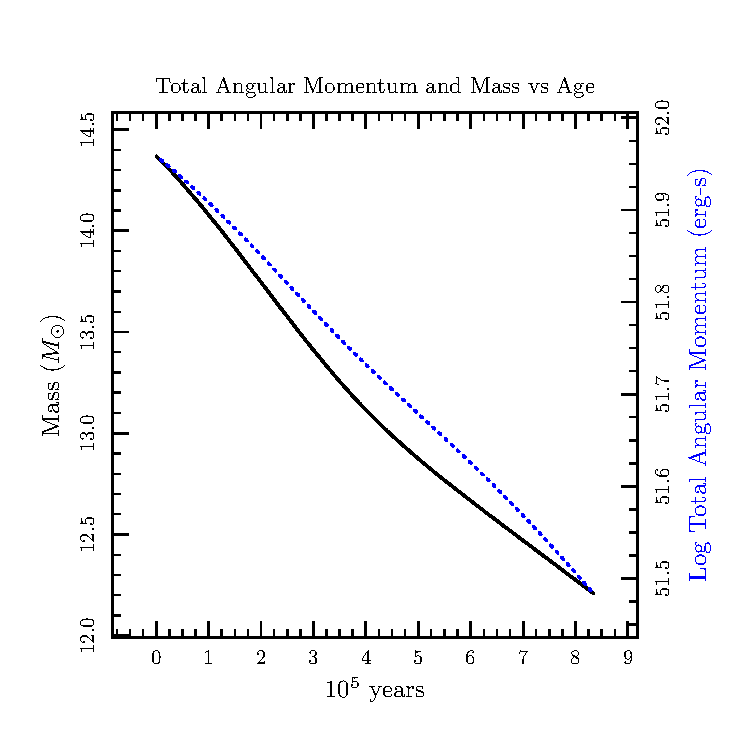
\includegraphics[width = 3.8in]{/Users/jaredbrooks/15M_dynamo/plots_out/Total_Angular_Momentum_vs_Age.pdf}
		       \caption{Mass and Total Angular Momentum vs Age plot}
		       \label{fig:1}
                \end{minipage}
                \hspace{0cm}
                \begin{minipage}[b]{0.5\linewidth}
                       \centering
                       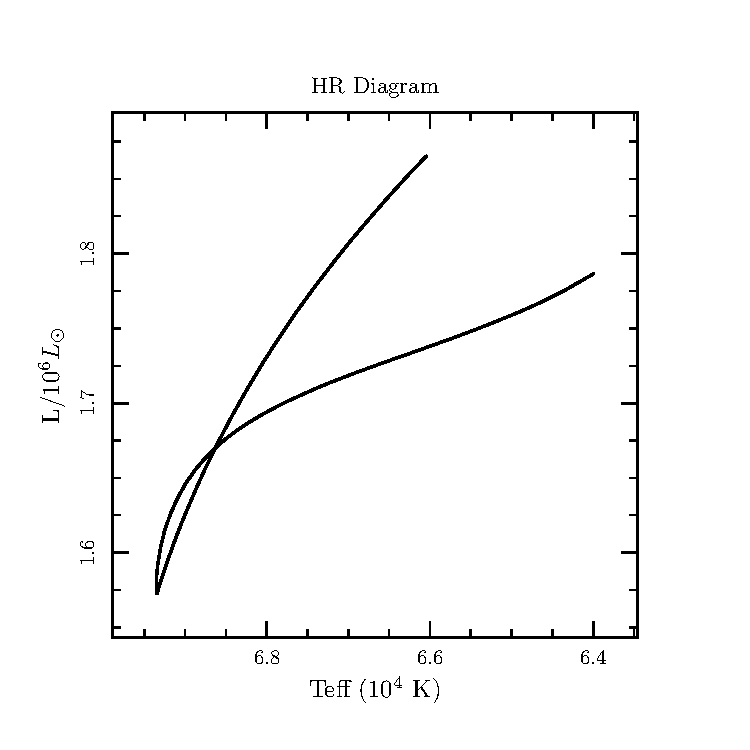
\includegraphics[width = 3.8in]{/Users/jaredbrooks/15M_dynamo/plots_out/HR_Diagram.pdf}
                       \caption{H.R. Diagram, evolution starts on top branch}
                       \label{fig:2}
                \end{minipage}
	\end{figure}

        \pagebreak

        The evolution of the surface rotation of the star is shown in figure \ref{fig:3}. Both the equatorial rotational velocity ($v_{surf}$) and the ratio of angular velocity to the critical angular velocity\footnote{The critical angular velocity ($\Omega_{crit}$) is the rotation rate at which the sum of centrifugal and radiation force cancel out gravity} at the surface ($\Omega/\Omega_{crit}$) are plotted.  The evolution of these variables is a consequence of the approximate conservation of angular momentum as the star expands and contracts.  A profile showing the dominant diffusion processes in the last  model calculated by the test is presented in figure \ref{fig:4}. The Eddington-Sweet and Goldreich-Schubert-Fricke rotational diffusion and Spruit-Taylor magnetic diffusion are the dominant mixing processes in the radiative region of the star. This radiative region is located between the convective core (burning He) and the convective H-rich envelope. 

        \begin{figure}[H]
                \begin{minipage}[b]{0.5\linewidth}
                       \centering
                       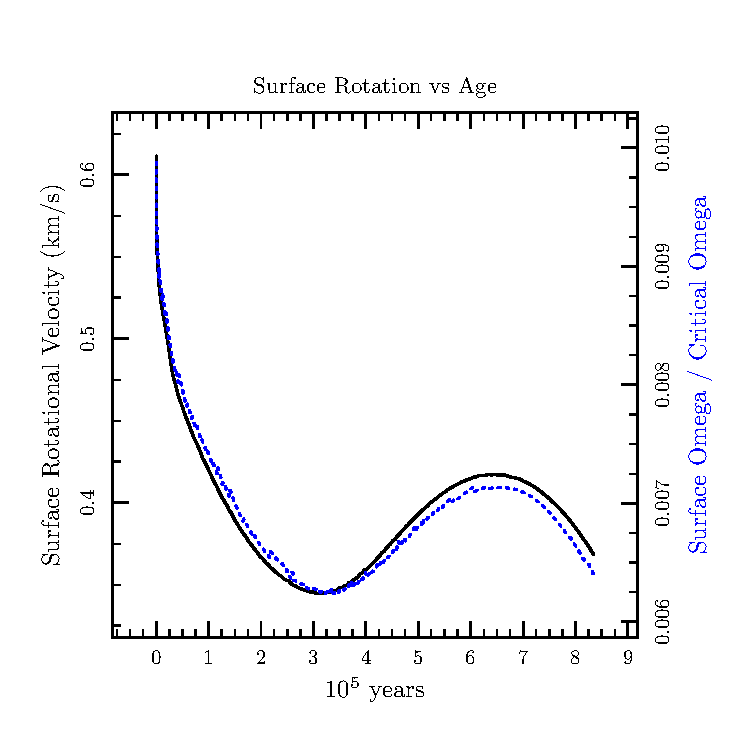
\includegraphics[width = 3.8in]{/Users/jaredbrooks/15M_dynamo/plots_out/Surface_Rotation_vs_Age.pdf}
                       \caption{Surface Rotation vs Age plot}
                       \label{fig:3}
                \end{minipage}
                \hspace{0cm}
                \begin{minipage}[b]{0.5\linewidth}
                       \centering
                       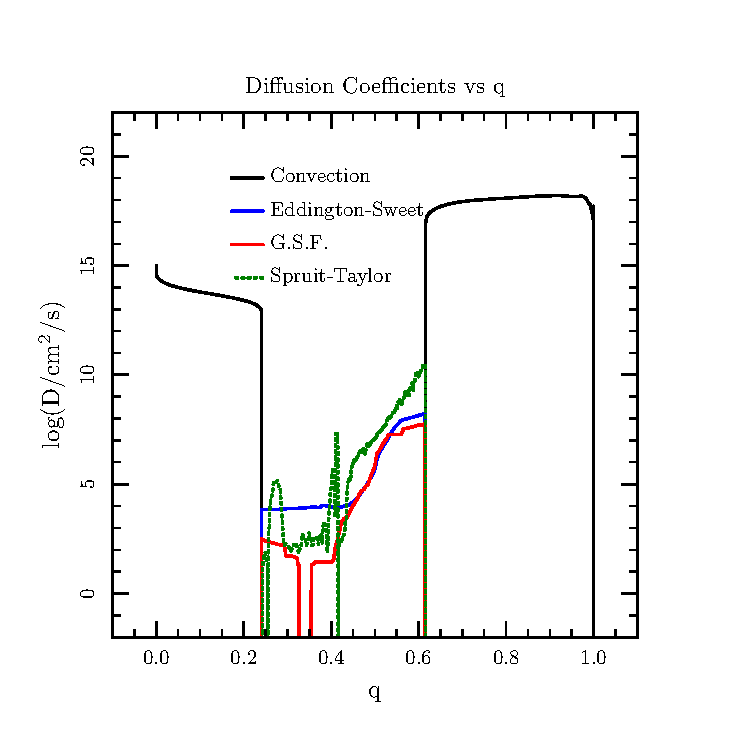
\includegraphics[width = 3.8in]{/Users/jaredbrooks/15M_dynamo/plots_out/Diffusion_Coefficients_vs_q.pdf}
                       \caption{Diffusion coefficients calculated for the last model in the test}
                       \label{fig:4}
                \end{minipage}
        \end{figure}

        \pagebreak

        The following two profiles show the magnetic fields generated by the Taylor-Spruit dynamo in the poloidal (radial) and toroidal (azimuthal) components.  The profile to the left (figure \ref{fig:5}) shows that these magnetic fields are only being generated in the radiative region between convection zones.  The profile to the right (figure \ref{fig:6}) shows how magnetic field generation, especially in the toroidal component, is affected by rotation rate.

        \begin{figure}[H]
                \begin{minipage}[b]{0.5\linewidth}
                       \centering
                       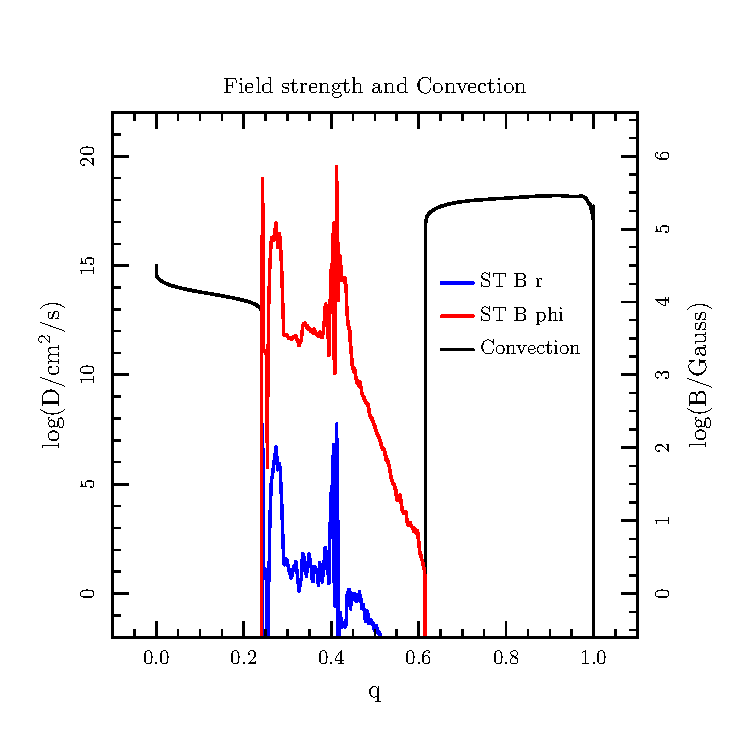
\includegraphics[width = 3.8in]{/Users/jaredbrooks/15M_dynamo/plots_out/B_and_Conv_vs_q.pdf}
                       \caption{Magnetic fields generated in radiative region}
                       \label{fig:5}
                \end{minipage}
                \hspace{0cm}
                \begin{minipage}[b]{0.5\linewidth}
                       \centering
                       \includegraphics[width = 3.8in]{/Users/jaredbrooks/15M_dynamo/plots_out/B_and_Omega_vs_q.pdf}
                       \caption{Magnetic field generation limited by rotation rate}
                       \label{fig:6}
                \end{minipage}
        \end{figure}

        \pagebreak

        At the beginning of the run we see from the abundance profile (figure \ref{fig:10}) that the core is made up of mainly helium, with nitrogen being the next most abundant element in the core.  The burning rate profile at the beginning of the run (figure \ref{fig:11}) shows that triple alpha and nitrogen burning are dominant in the core, with CNO burning dominant just outside the core.  Abundances and burning rates are plotted against q, where q is the fraction of star mass interior to outer boundary of each zone, moving outwards from the core.

        \begin{figure}[H]
                \begin{minipage}[b]{0.5\linewidth}
                       \centering
                       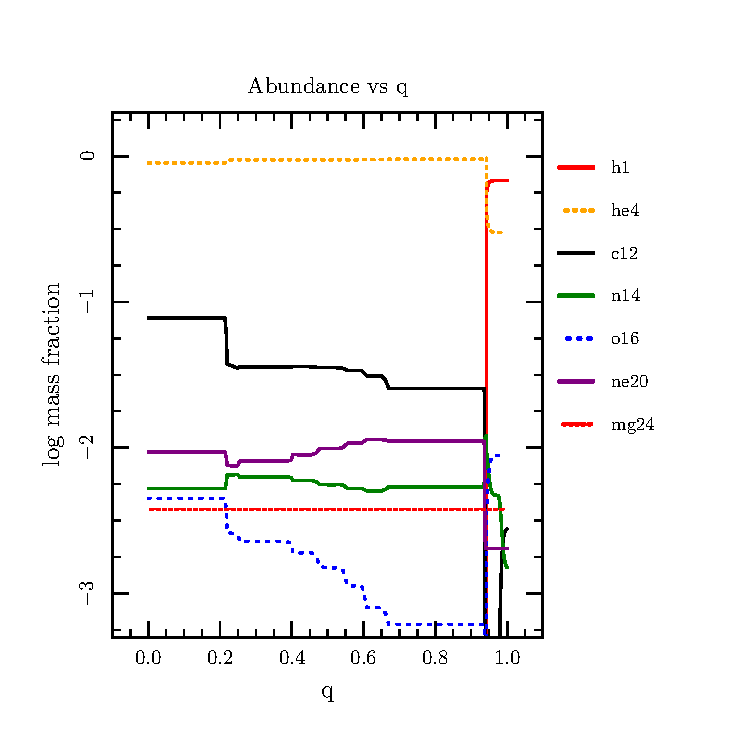
\includegraphics[width = 3.8in]{/Users/jaredbrooks/15M_dynamo/plots_out/Abundance_vs_q_1.pdf}
                       \caption{Abundance profile at beginning, helium core}
                       \label{fig:10}
                \end{minipage}
                \hspace{0cm}
                \begin{minipage}[b]{0.5\linewidth}
                       \centering
                       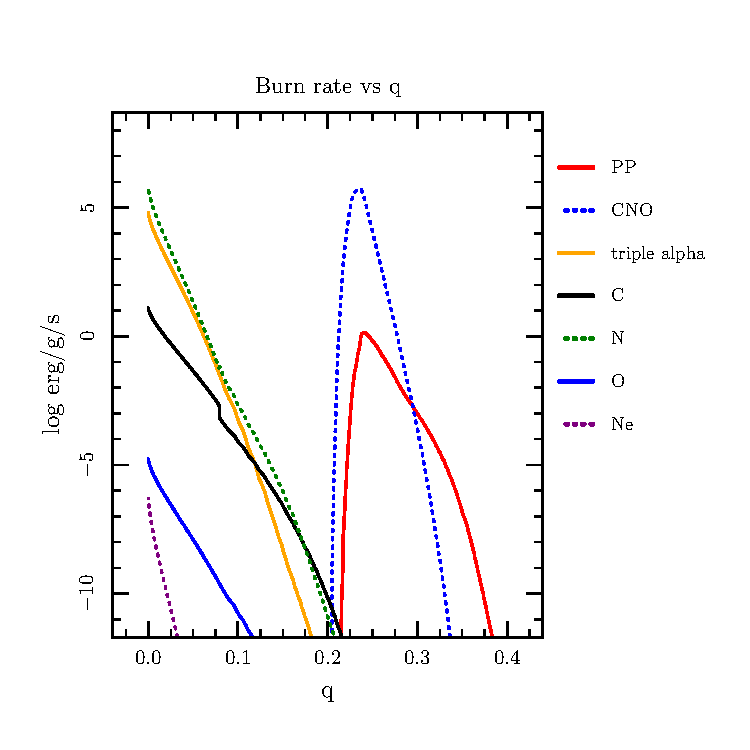
\includegraphics[width = 3.8in]{/Users/jaredbrooks/15M_dynamo/plots_out/Burnrate_vs_q_1.pdf}
                       \caption{Burning rate profile, triple alpha and nitrogen dominant}
                       \label{fig:11}
                \end{minipage}
        \end{figure}

        \pagebreak

        By the end of the run we see from the abundance profile (figure \ref{fig:12}) that hydrogen in the core has been burned into heavier elements, mainly carbon and oxygen.  From the burning rate profile taken at the end of the run (figure \ref{fig:13}), we can see that carbon and triple alpha burning are dominant in the core, and CNO burning has been push out to approximately q = 0.4.

        \begin{figure}[H]
                \begin{minipage}[b]{0.5\linewidth}
                       \centering
                       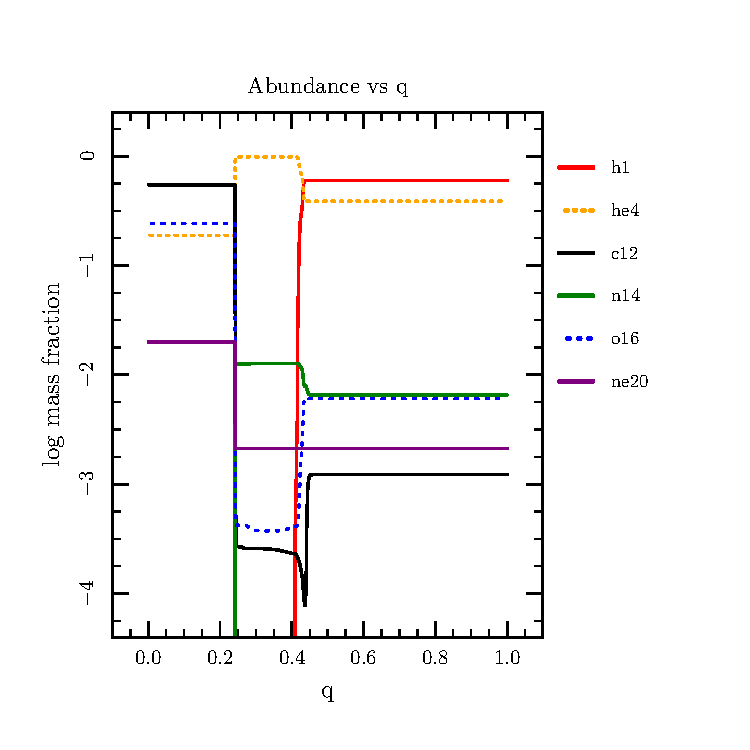
\includegraphics[width = 3.8in]{/Users/jaredbrooks/15M_dynamo/plots_out/Abundance_vs_q_9.pdf}
                       \caption{Abundance profile at end, carbon-oxygen core}
                       \label{fig:12}
                \end{minipage}
                \hspace{0cm}
                \begin{minipage}[b]{0.5\linewidth}
                       \centering
                       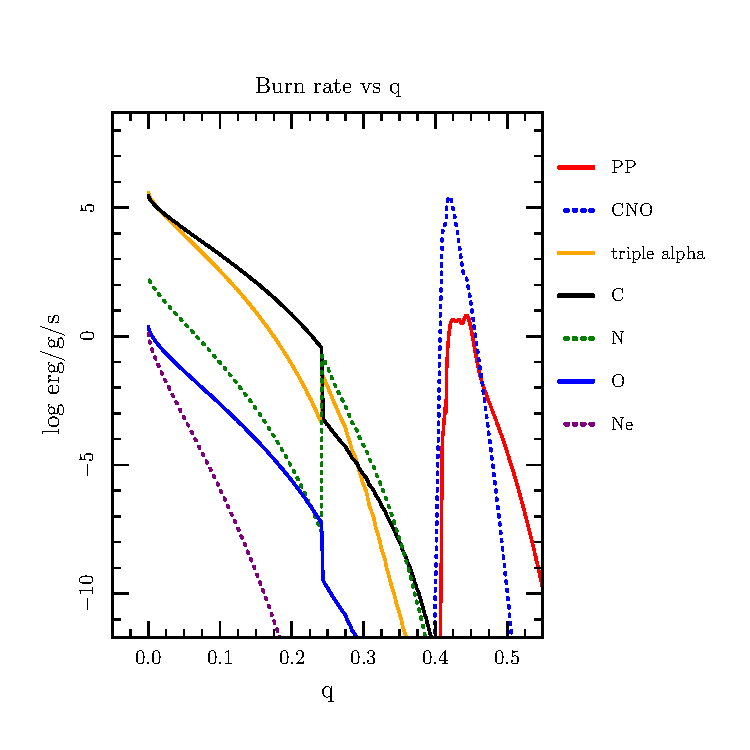
\includegraphics[width = 3.8in]{/Users/jaredbrooks/15M_dynamo/plots_out/Burnrate_vs_q_9.pdf}
                       \caption{Burning rate profile, carbon and triple alpha dominant}
                       \label{fig:13}
                \end{minipage}
        \end{figure}

        \pagebreak

        This final plot (figure \ref{fig:7}) is meant to show a few internal \texttt{MESA} variables, such as the size of the time-step, the number of zones, and the number of retries against the model number in order to give some understanding of how hard \texttt{MESA} is working throughout the run and where some areas of problems/interest might be.

        \begin{figure}[H]
                \centering
                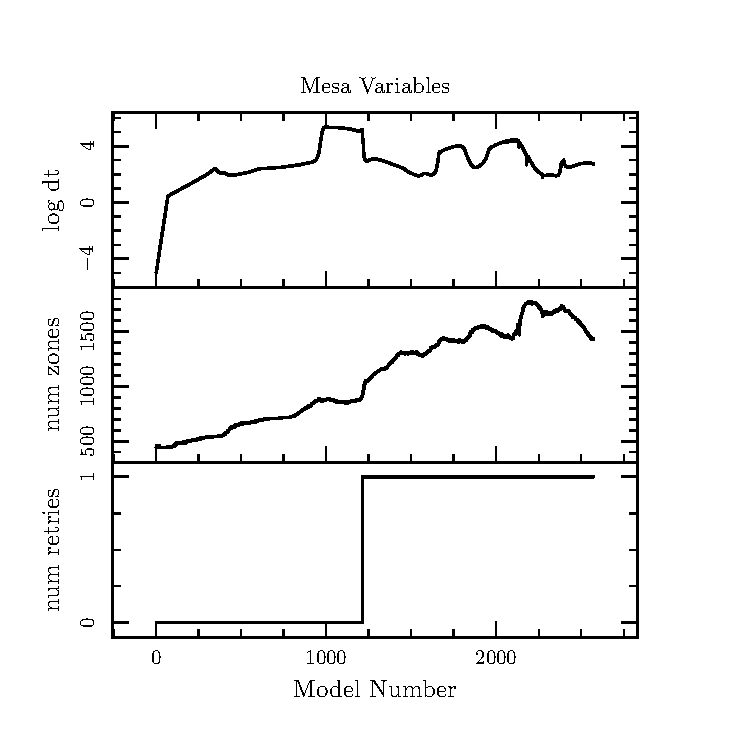
\includegraphics[width = 5in]{/Users/jaredbrooks/15M_dynamo/plots_out/Mesa_Variables.pdf}
                \caption{\texttt{MESA} variables plotted against model number show how hard \texttt{MESA} is working}
                \label{fig:7}
        \end{figure}

\end{document}


